%%
%% The official i6 slide template _demo_
%% created by Philippe Dreuw and Thomas Deselaers, 2005
%%
%% $Id: slides.tex,v 1.48 2007-11-14 17:13:01 dreuw Exp $
%%
%% Possible options for:
%%  - language       : 'english' (default), 'german'
%%  - page numbering : 'nonumber', 'lastpage' to enable automatic page n/m numbering, 
%%                     'userlastpage' to enable a user defined page n/m numbering using \LastPage command,  
%%                      or leave empty for normal page numbering (default)
%%  - itemize        : 'triangle' or leave empty for bullets (default)
%%  - page titles    : 'allowpagebreaks' to enable titles with automatic page breaks, 
%%                     'nopagebreaks' to disable (default)
%%  - page layout    : 'vertical' to enable vertical centering on each slide using \vfill ... \vfill (default)
%%  - encoding       : 'utf-8' to enable utf encoding instead of latin1 (default)
%%  - tools          : 'blackslide' to insert a black slide which is linked with every slide title, e.g. to write a proof on the blackboard
%%
\documentclass[11pt, a4paper, landscape]{article}
\usepackage{NeyDreuwSlides_Oct08}

\usepackage{amsthm}
\newtheorem{definition}{Definition}
\newtheorem{theorem}{Theorem}[section]
\usepackage{algorithm}
\usepackage{algpseudocode}
\renewcommand{\algorithmicrequire}{\textbf{Input:}}
\renewcommand{\algorithmicensure}{\textbf{Output:}}

%%%%%%%%%%%%%%%%%%%%%%%%%%%%%%%%%%%%%%%%%%%%%%%%%%%%%%%%%%%%%%%%%%%%%%%%%%%%%%%%
%% flyspell can read the local ispelldict variable to automatically change the dictionary, 
%% e.g. german-new8, american, english, british, ...
%% 
%% Local IspellDict: american
%% 


%%%%%%%%%%%%%%%%%%%%%%%%%%%%%%%%%%%%%%%%%%%%%%%%%%%%%%%%%%%%%%%%%%%%%%%%%%%%%%%%
% custom packages
\usepackage{fancyvrb} %%% fancy verbatim to enable coloring within verbatim environments

%\usepackage{pst-node} 

%%%%%%%%%%%%%%%%%%%%%%%%%%%%%%%%%%%%%%%%%%%%%%%%%%%%%%%%%%%%%%%%%%%%%%%%%%%%%%%%
% Some example hacks work only in combination with the 'pdflatex -shell-escape'
% mode. Try 'make hacks'


%%%%%%%%%%%%%%%%%%%%%%%%%%%%%%%%%%%%%%%%%%%%%%%%%%%%%%%%%%%%%%%%%%%%%%%%%%%%%%%%
\renewcommand*{\title}{Graph-Based Image Segmentation}        % main title of the work (used for \TitlePage)
\renewcommand*{\titleshort}{Graph-Based Segmentation}         % short title (used for \lfoot)
\renewcommand*{\occasion}{Seminar Medical Image Processing -- MedBV13}		% (used for \TitlePage)
\renewcommand*{\occasionshort}{MedBV13}               % short occasion title (used for \rfoot)
%\renewcommand*{\date}{11. April 2005}                                        % default is \today (used for \TitlePage and \rfoot)
\renewcommand*{\author}{Phan-Anh Nguyen, Christian Oberdoefer}         % all the authors of the work, can be long (used for \TitlePage)
\renewcommand*{\authorshort}{Phan-Anh et al.:\xspace}                            % all the authors of the work, should be short (used for \lfoot)
\renewcommand*{\email}{\url{anh.nguyen@rwth-aachen.de, oberdoefer@i6.informatik.rwth-aachen.de}}  % all email address(es) of the authors (used for \TitlePage)
\renewcommand*{\mainauthor}{Phan-Anh Nguyen}                                   % the author(s) who presented the work (used for \TitlePage)
\renewcommand*{\mainauthoremail}{\url{anh.nguyen@rwth-aachen.de}}    % presenter mail address(es) (used for \FinalPage)
\renewcommand*{\www}{http://www-i6.informatik.rwth-aachen.de/}                % web address (used for \TitlePage _and_ \FinalPage)
\newcommand*{\keywords}{Graph Cut, Segmentation}                               % keywords, can be used for PDF summary

% will be set into the PDF document summary
\hypersetup{
  pdftitle={\title}, 
  pdfsubject={\occasion},  
  pdfauthor={\author}, 
  pdfkeywords={\keywords},
  % enable automatic page transitions: for endless loop edit in
  % acrobat reader -> preferences -> full screen -> after every X
  % seconds and after last page
  pdfpageduration = 2, 
%  pdfpagetransition = {Glitter /Di 315 /D 5}  
  pdfpagetransition = {Box /M /O /D 1},
}

%%%%%%%%%%%%%%%%%%%%%%%%%%%%%%%%%%%%%%%%%%%%%%%%%%%%%%%%%%%%%%%%%%%%%%%%%%%%%%%%
\listfiles
%%%%%%%%%%%%%%%%%%%%%%%%%%%%%%%%%%%%%%%%%%%%%%%%%%%%%%%%%%%%%%%%%%%%%%%%%%%%%%%%
\begin{document}

%%%%%%%%%%%%%%%%%%%%%%%%%%%%%%%%%%%%%%%%%%%%%%%%%%%%%%%%%%%%%%%%%%%%%%%%%%%%%%%%
\TitlePage

%%%%%%%%%%%%%%%%%%%%%%%%%%%%%%%%%%%%%%%%%%%%%%%%%%%%%%%%%%%%%%%%%%%%%%%%%%%%%%%%
\NewPage\headline{Outline}
%\small
\vfill
\begin{enumerate}
\item \hyperlink{sli:introduction}{Introduction and Motivation}
\item \hyperlink{sli:features}{Image Features}
%\begin{itemize}
%	\item \hyperlink{sli:surf}{Speeded Up Robust Features}
%	\item \hyperlink{sli:gPb}{Globalized Probability of Boundary}
%\end{itemize}
\item \hyperlink{sli:supervised}{Segmentation with Supervised Training}
%\begin{itemize}
%	\item \hyperlink{sli:svm}{Support Vector Machine for Region Ranking}
%	\item \hyperlink{sli:logistic}{Logistic Regression}
%	\item \hyperlink{sli:ssm}{Statistical Shape Model}
%\end{itemize}
\item \hyperlink{sli:construction}{Graph Construction}
%\begin{itemize}
%	\item \hyperlink{sli:region_graph}{Region Graph}
%	\item \hyperlink{sli:contour_graph}{Contour Graph}
%	\item \hyperlink{sli:mrf}{Markov Random Field}
%\end{itemize}
\item \hyperlink{sli:algorithms}{Graph Cut Algorithms}
%\begin{itemize}
%	\item \hyperlink{sli:PCST}{Prize-Collecting Steiner Tree}
%	\begin{itemize}
%		\item \hyperlink{sli:branch_and_cut}{Branch-and-Cut Algorithm}
%	\end{itemize}
%	\item \hyperlink{sli:contour_cut}{Contour Cut}
%	\begin{itemize}
%		\item \hyperlink{sli:circulation}{Graph Circulations}
%		\item \hyperlink{sli:cost}{The Cost Function}
%		\item \hyperlink{sli:solution}{Computational Solution}
%	\end{itemize}
%	\item \hyperlink{sli:graph_cut}{Graph-Cut}
%	\begin{itemize}
%		\item \hyperlink{sli:min_cut}{Min-Cut Algorithm}
%		\item \hyperlink{sli:multi_shape}{Multi-Shape Graph-Cuts}
%	\end{itemize}
%\end{itemize}
\item \hyperlink{sli:application}{Applications}
%\begin{itemize}
%	\item \hyperlink{sli:ERS}{Efficient Region Search for Object Detection}
%	\item \hyperlink{sli:contour_detector}{Salient Contour Detection}
%	\item \hyperlink{sli:lung_segmentation}{Multi-Shape Graph-Cut for Lung Segmentation}
%\end{itemize}
\item \hyperlink{sli:conclusion}{Conclusion}
\end{enumerate}
\vfill
%\centerline{\footnotesize PS: the outline should not have more than 5-7 items
%  without any subitems}
%\normalsize
%\vfill


%%%%%%%%%%%%%%%%%%%%%%%%%%%%%%%%%%%%%%%%%%%%%%%%%%%%%%%%%%%%%%%%%%%%%%%%%%%%%%%%
\NewPage\headline{Literature} 
\vfill 
\begin{itemize}
\item S. Vijayanarasimhan and K. Grauman. \alert{Efficient region search for object detection.} Computer Vision and Pattern Recognition (CVPR), 2011 IEEE Conference, pages 1401--1408, June 2011.
\item R. Kennedy, J. Gallier, and Jianbo Shi. \alert{Contour cut: Identifying salient contours in images
by solving a hermitian eigenvalue problem.} Computer Vision and Pattern Recognition (CVPR), 2011 IEEE Conference, pages 2065--2072, June 2011.
\item Nakagomi, K. and Shimizu, A. and Kobatake, H. and Yakami, M. and Fujimoto, K. and Togashi, K. \alert{Multi-shape graph-cuts and its application to lung segmentation from a chest CT volume.} Fourth International Workshop on Pulmonary Image Analysis, 2011.
\end{itemize}
\nocite{*}
\vfill





%%%%%%%%%%%%%%%%%%%%%%%%%%%%%%%%%%%%%%%%%%%%%%%%%%%%%%%%%%%%%%%%%%%%%%%%%%%%%%%%
\NewPage\headline{Introduction and Motivation} 
\hypertarget{sli:introduction}
\normalsize
\vfill
\begin{itemize}
	\item Purposes of segmentation
	\begin{itemize}
		\item Computer-aided diagnoses:\\
		measure object's size and shape.
		\item Mobile robots: scene understanding.
	\end{itemize}
	\item Current problems
	\begin{itemize}
		\item Deformable shapes
		\item Time constraint
		\item No clear boundaries
	\end{itemize}
	\item Advantages of graph representation
	\begin{itemize}
		\item Can be transformed into standard graph problems
		\item Can be solved efficiently
		\item Optimal solution possible
	\end{itemize}
\end{itemize}
%\begin{figure}
%	\centering
%	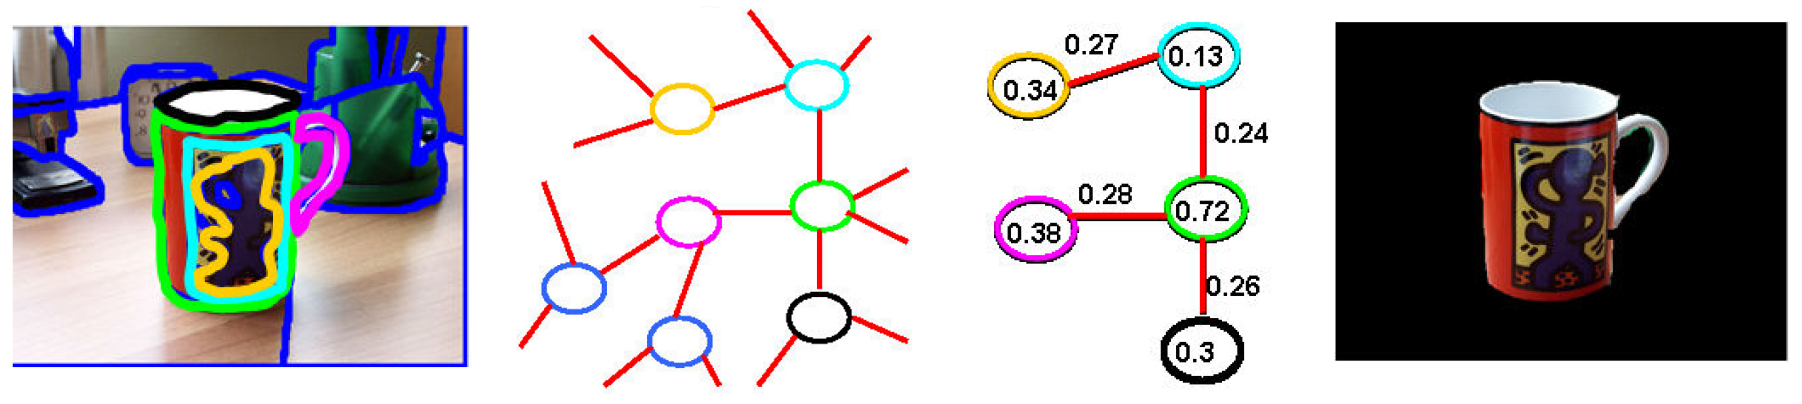
\includegraphics[width=.5\linewidth]{region_graph_intro}
%\end{figure}
\begin{textblock}{3}(21,-15)
  \scalebox{0.35}{\includegraphics{region_graph_intro1}}
\end{textblock} 
\begin{textblock}{3}(21,-11.5)
  \scalebox{0.3}{\includegraphics{region_graph_intro2}}
\end{textblock} 
\begin{textblock}{3}(22,-7)
  \scalebox{0.4}{\includegraphics{region_graph_intro3}}
\end{textblock} 
\begin{textblock}{3}(21,-2.5)
  \scalebox{0.35}{\includegraphics{region_graph_intro4}}
\end{textblock} 
\vfill


%%%%%%%%%%%%%%%%%%%%%%%%%%%%%%%%%%%%%%%%%%%%%%%%%%%%%%%%%%%%%%%%%%%%%%%%%%%%%%%%
\NewPage\headline{Image Features}
\vfill
\begin{itemize}
\item Advantages:
\begin{itemize}
\item Capture important properties in local regions
\item Compact representation: High dimensional vectors
\item Computational effort: Very efficient
\item Invariant to: Translation, rotation, scaling, brightness.
\end{itemize}
\vfill
\item Point features: Speeded Up Robust Features (SURF)
\item Shape features:
\begin{itemize}
	\item Detector: Globalized Probability of Boundary (gPb)
	\item Shape descriptor
\end{itemize}
\end{itemize}
\vfill


%%%%%%%%%%%%%%%%%%%%%%%%%%%%%%%%%%%%%%%%%%%%%%%%%%%%%%%%%%%%%%%%%%%%%%%%%%%%%%%%
\NewPage\headline{Image Features: Speeded Up Robust Features}
\hypertarget{sli:style}
\vfill
\begin{enumerate}
\item Detect interest points: $det(Hessian(I)) = I_{xx}I_{yy} - I^2_{xy}$ at scale $s$
\item Orientation assignment (rotation invariant):
\begin{itemize}
\item Compute Haar wavelet responses $(d_x, d_y)$ within $6s$ around interest point.
\item Select dominant direction
\end{itemize}
\item SURF is computed within a window of size $20s$.
\end{enumerate}
\begin{table}
  \centering
  \begin{tabular}{@{} M{.3\linewidth} M{.3\linewidth} M{.3\linewidth} @{}}
      \includegraphics[width=0.25\textwidth]{feature_neighborhood}
      &
      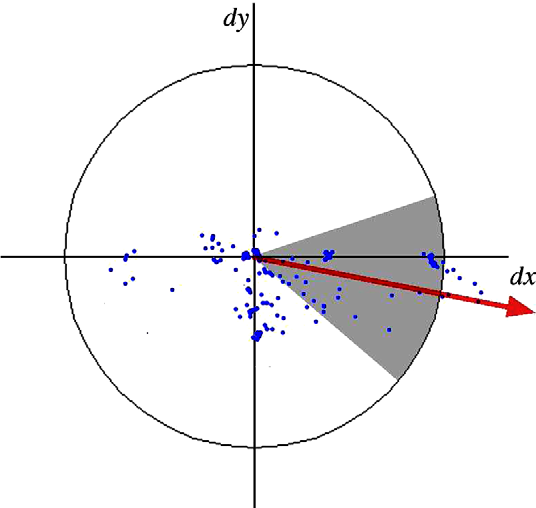
\includegraphics[width=0.3\textwidth]{orientation_window}%
      &
      
\includegraphics[width=0.2\textwidth]{haar_wavelet}%
  \end{tabular}
\end{table}
\vfill







%%%%%%%%%%%%%%%%%%%%%%%%%%%%%%%%%%%%%%%%%%%%%%%%%%%%%%%%%%%%%%%%%%%%%%%%%%%%%%%%
\NewPage\headline{Image Features: Speeded Up Robust Features}
\vfill
\begin{itemize}
\item Split the window into $4 \times 4$ sub-windows.
\item 4D descriptor vector $v = (\sum d_x, \sum d_y, \sum \lvert d_x \rvert, \sum \lvert d_y \rvert)$ for each sub-window\\
$\Rightarrow$ 64D SURF descriptor.
\item Normalize to make it invariant to brightness.
\item Invariant to: Translation, Scaling, Rotation, Brightness.
%\item[]
\end{itemize}
\begin{table}
  \centering
  \begin{tabular}{@{} M{.5\linewidth} M{.5\linewidth} @{}}
      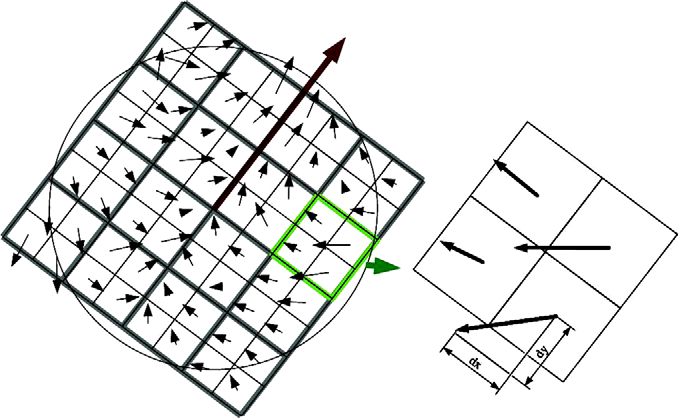
\includegraphics[width=0.4\textwidth]{surf}
      &
      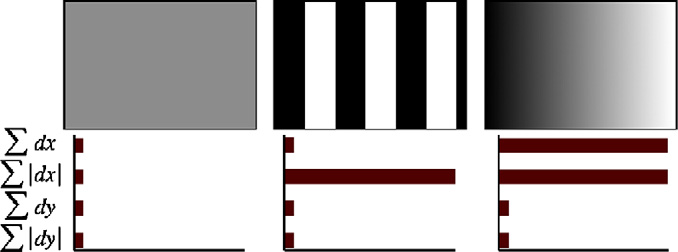
\includegraphics[width=0.4\textwidth]{surf_vector}%
  \end{tabular}
\end{table}
\vfill





%%%%%%%%%%%%%%%%%%%%%%%%%%%%%%%%%%%%%%%%%%%%%%%%%%%%%%%%%%%%%%%%%%%%%%%%%%%%%%%%
\NewPage\headline{Image Features: Gradient-based Detector}
\small
\vfill
\begin{enumerate}
\item Draw a circle with radius $r$, divide it along the diameter at orientation $\theta$.
\item Build histograms of brightness, color and texture for each disc half: $h$ and $g$.
\item Compares histograms of the two disc halves: $G(x, y, \theta, r) = \chi ^ 2 (g, h) = \frac{1}{2} \sum_i \frac{(g_i - h_i)^2}{(g_i + h_i)}$.
%\item Use logistic regression trained on human segmentation dataset to get the result $Pb_{\sigma}(x, y, \theta)$.
\end{enumerate}
\begin{figure}
	\centering
	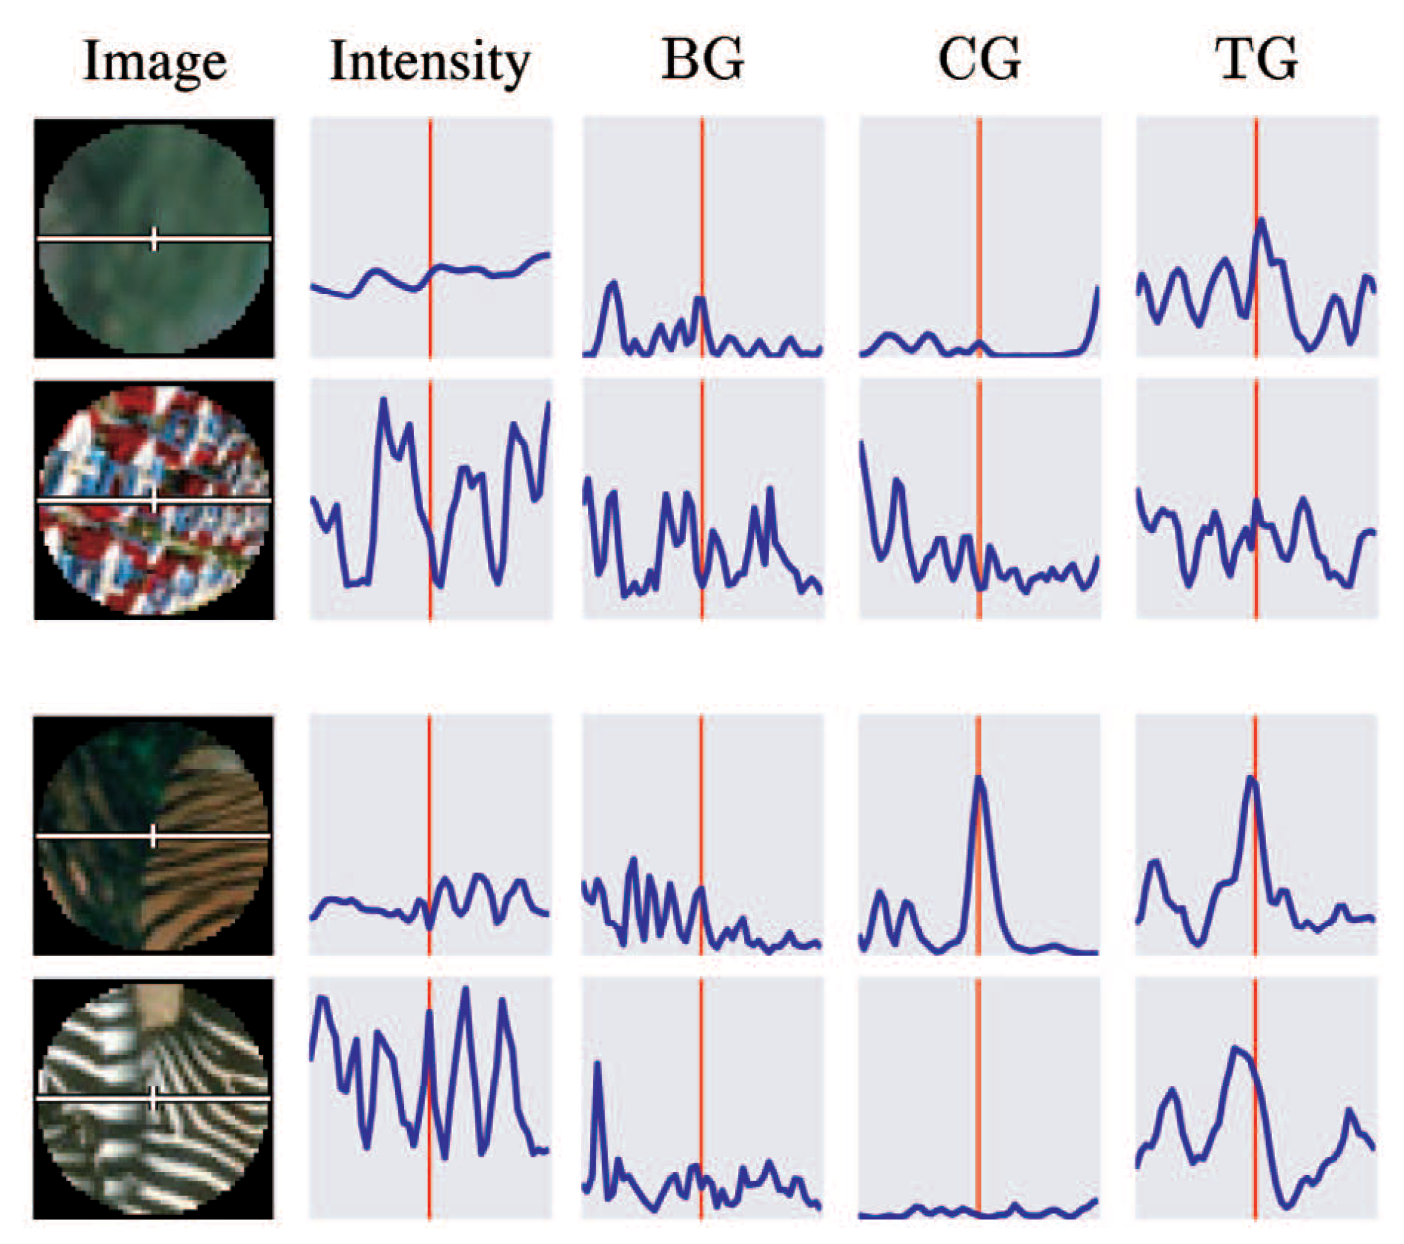
\includegraphics[width=0.45\textwidth]{gradient_features}
\end{figure}
\vfill


%%%%%%%%%%%%%%%%%%%%%%%%%%%%%%%%%%%%%%%%%%%%%%%%%%%%%%%%%%%%%%%%%%%%%%%%%%%%%%%%
\NewPage\headline{Globalized Probability of Boundary Detector}
\small
\vfill
\begin{itemize}
\item Brightness, color and texture gradients in 3 different scales: $mPb(x, y, \theta) = \sum\limits_{i = 1}^{9} G_i(x, y, \theta)$.
\item Define affinity matrix $W$ using intervening contour cue $mPb$.
\item Solve the generalized eigenvectors problem: $(D - W)v = \lambda D v$, $D_{ii} = \sum_j W_{ij}$\\ to get top $k$ eigenvectors $v_j$.
\item Extract edges from $v_j$ to get $sPb_{v_j}(x, y, \theta)$: $sPb(x, y, \theta) = \sum\limits_{j = 1}^{k} \frac{1}{\sqrt{\lambda_j}} sPb_{v_j} (x, y, \theta)$.
\item Globalized probability of boundary: $gPb(x, y, \theta) = \sum\limits_{i = 1}^{9} \beta_iG_i(x, y, \theta) + \gamma sPb(x, y, \theta)$.
\end{itemize}
%  \begin{figure}
%    \centering
%    \begin{tabularx}{600pt}{Z Z}
%      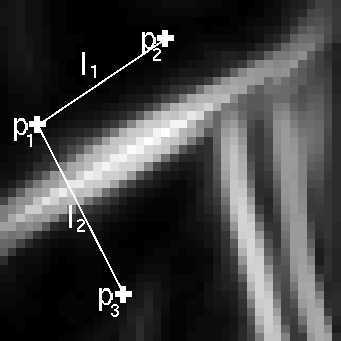
\includegraphics[width=0.15\textwidth]{intervening_contour2}%
%      \caption{Intervening contour}%
%      &
%      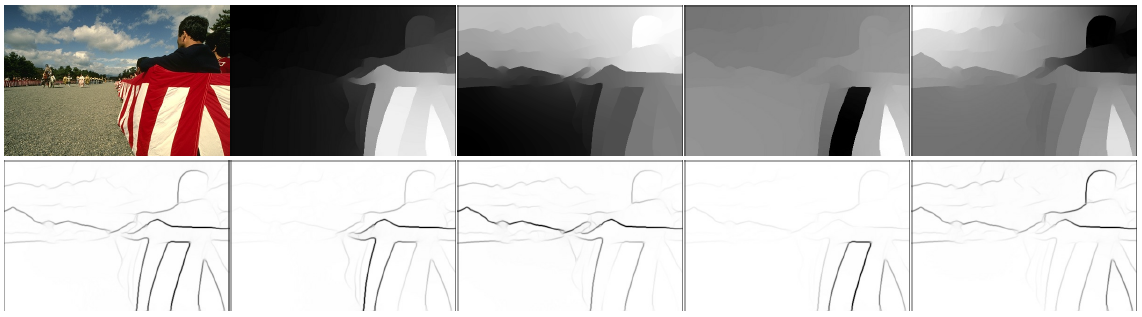
\includegraphics[width=0.55\textwidth]{sPb}%
%      \caption{Eigenvectors and their edges}%
%    \end{tabularx}
%  \end{figure}
\begin{table}
  \centering
  \begin{tabular}{@{} M{.3\linewidth} M{.7\linewidth} @{}}
      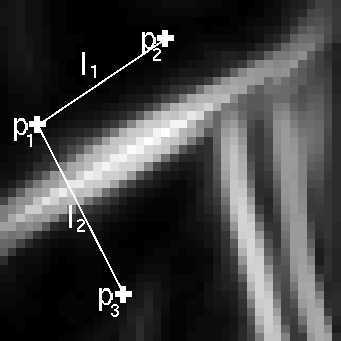
\includegraphics[width=0.15\textwidth]{intervening_contour2}%
      %\caption{Intervening contour}%
      &
      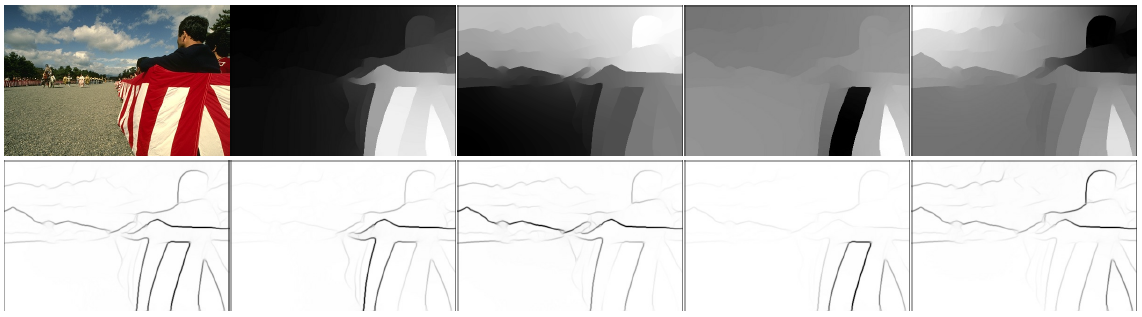
\includegraphics[width=0.65\textwidth]{sPb}%
      %\caption{Eigenvectors and their edges}%
  \end{tabular}
\end{table}
\vfill


%%%%%%%%%%%%%%%%%%%%%%%%%%%%%%%%%%%%%%%%%%%%%%%%%%%%%%%%%%%%%%%%%%%%%%%%%%%%%%%%
\NewPage\headline{Image Features: Shape Descriptor}
\vfill
\begin{itemize}
\item Split region's bounding box into $4 \times 4$ grid.
\item Different features are extracted from the cells:
\begin{itemize}
\item Contour shape, given by the histogram of oriented responses of the contour detector $gPb$
\item Edge shape, computed by convolution with a [-1 0 1] filter along $x$ and $y$ axes
\item Color, represented by the $L^*$, $a$ and $b$ histograms in the CIELAB color space
\item Texture, described by texton histograms
\end{itemize}
\item Each type of cue is encoded by concatenating cell signals into a histogram.
\begin{itemize}
\item 8 orientations for gPb contours
\item At least 2 dimensions for edge
\item 3D histogram for color
\item 200 dimensions for textures
\end{itemize}
\end{itemize}
\vfill


%%%%%%%%%%%%%%%%%%%%%%%%%%%%%%%%%%%%%%%%%%%%%%%%%%%%%%%%%%%%%%%%%%%%%%%%%%%%%%%%
\NewPage\headline{Supervised Training: Support Vector Machine}
\vfill
\begin{itemize}
\item Given training data $\left\lbrace (h_i, t_i) \right\rbrace _{i = 1} ^S$, find a classifier $f(h) = w^Th + b$ that maximizes the margin.
\vfill
\item Equivalent to find a hyperplane satisfying: $\arg\min\limits_{w, b} \frac{1}{2} \|w\| ^2,$ subject to $t_i(w^Th_i + b) \geq 1 \forall i$.
\vfill
\item The solution for $w$ is a linear combination of training examples: $w = \sum\limits_{i = 1}^{S} a_it_ih_i = \sum\limits_{i = 1}^{S} \alpha_ih_i$.
\end{itemize}
\begin{figure}
	\centering
	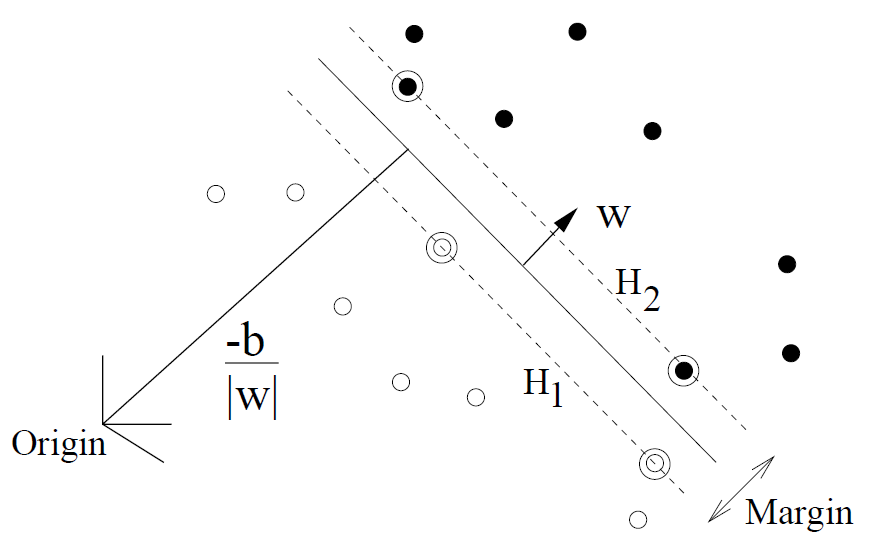
\includegraphics[width=0.5\textwidth]{svm}
\end{figure}
\vfill


%%%%%%%%%%%%%%%%%%%%%%%%%%%%%%%%%%%%%%%%%%%%%%%%%%%%%%%%%%%%%%%%%%%%%%%%%%%%%%%%
\NewPage\headline{SVM for Region Ranking}
\vfill
\begin{figure}
	\centering
	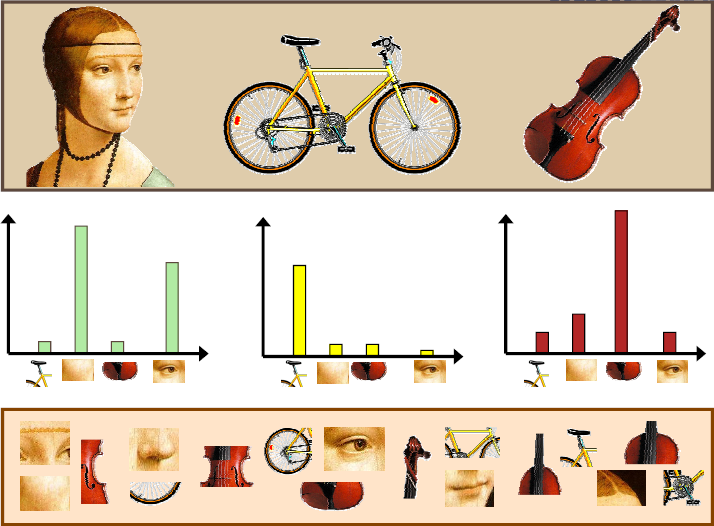
\includegraphics[width=0.35\textwidth]{bag_of_features}
	%\caption{Bag of visual words}
\end{figure}
\begin{itemize}
\item Given region $R = \left\lbrace (x_i, v_i) \right\rbrace _{i = 1} ^N$, its ranking score:
\begin{equation*}
\begin{array}{lcl}
f(R) & = & b + (\sum\limits_{i = 1}^{S}\alpha_ih(R_i)) \cdot h(R)\\
     & = & b + \sum\limits_{i = 1}^{S}\sum\limits_{j = 1}^{K} \alpha_ih_j(R_i)h_j(R)\\
     %& = & b + \sum\limits_{j = 1}^{K}\sum\limits_{i = 1}^{S} \alpha_ih_j(R_i)h_j(R)\\
     & = & b + \sum\limits_{j = 1}^{K} w_jh_j(R) = b + \sum\limits_{i = 1}^{N} w_{d_i}
\end{array}
\end{equation*}
\item $d_i \in \left[ 1, K \right] $ the index of the visual word that feature $v_i$ maps to.
\end{itemize}
\vfill


%%%%%%%%%%%%%%%%%%%%%%%%%%%%%%%%%%%%%%%%%%%%%%%%%%%%%%%%%%%%%%%%%%%%%%%%%%%%%%%%
\NewPage\headline{Graph Construction}
\vfill
\begin{itemize}
\item Region Graph
\begin{itemize}
\item Graph of Regions with arbitrary shape
\end{itemize}
\vfill
\item Contour Graph
\begin{itemize}
\item Graph of Edge segments
\end{itemize}
\vfill
\item Markov Random Field
\begin{itemize}
\item Voxel graph with shape priors
\end{itemize}
\end{itemize}
\vfill


%%%%%%%%%%%%%%%%%%%%%%%%%%%%%%%%%%%%%%%%%%%%%%%%%%%%%%%%%%%%%%%%%%%%%%%%%%%%%%%%
\NewPage\headline{Region Graph}
\vfill
\begin{itemize}
%\item Watershed to define regions from gPb contours
\item Vertex weights based on SVM on SURF and Shape descriptors
\item Edge weights based on intervening contour strengths
\item Given region $R = \left\lbrace (x_i, v_i) \right\rbrace _{i = 1} ^N \cup \left\lbrace v_j \right\rbrace _{j = 1} ^M$
\item Its ranking score $f^{\prime}(R) = \sum\limits_{i = 1}^{N}w^v_{d_i} - \sum\limits_{j = 1}^{M} w^e_{s_j}$
\item $s_j \in \left[ 1, L \right] $ is the bin index of the contour strength histogram for the $j^{th}$ contour.
\end{itemize}
\begin{figure}
	\centering
	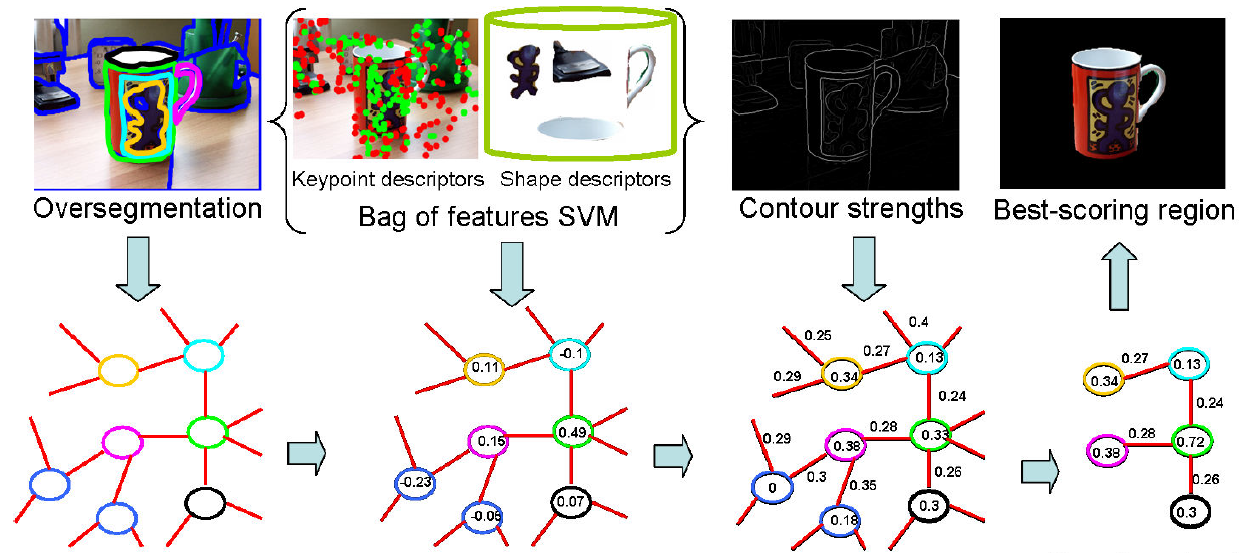
\includegraphics[width=0.75\textwidth]{region_graph}
\end{figure}
\vfill


%%%%%%%%%%%%%%%%%%%%%%%%%%%%%%%%%%%%%%%%%%%%%%%%%%%%%%%%%%%%%%%%%%%%%%%%%%%%%%%%
\NewPage\headline{Prize-Collecting Steiner Tree Problem}
\vfill
\begin{definition}
PCST PROBLEM: Given a connected undirected vertex and edge weighted graph G = (V, E, c, p) with vertex profits $p: V \rightarrow \mathbb{R}^{\geq 0}$ and edge costs $c: E \rightarrow \mathbb{R}^{\geq 0}$, find a connected subgraph T = ($V_T \subseteq V, E_T \subseteq E$) of G that maximizes the profit:
\begin{equation}
P(T) = \sum\limits_{v \in V_T} p(v) - \sum\limits_{e \in E_T} c(e)
\end{equation}
\end{definition}
\begin{itemize}
\item Optimal solution: branch-and-cut algorithm
\item Efficient for hundreds of nodes
\end{itemize}
\vfill


%%%%%%%%%%%%%%%%%%%%%%%%%%%%%%%%%%%%%%%%%%%%%%%%%%%%%%%%%%%%%%%%%%%%%%%%%%%%%%%%
\NewPage\headline{Contour Graph}
\vfill
\begin{itemize}
\item Threshold edge detector output to get edge segments: edgels.
\item Duplicate each edgel into $i$ and $\bar{i}$ with opposite directions $\theta, \theta + \pi$.
\item Connect pairs of edgels within some distance $r_e$: $E = \left\lbrace (i, j) : \| (x_i, y_i) - (x_j, y_j) \| \leq r_e \right\rbrace $.
\item Weights measure directed collinearity: $W_{ij} = e^{-(1 - cos(\mid \phi_i \mid + \mid \phi_j \mid))/\sigma^2}\ \mathrm{if}\ i \rightarrow j$.
\item Curve $\Rightarrow$ two chains $\Rightarrow$ convert into a cycle by adding an edge between terminal points.
\item Circulation $F = \Pi P$, where $P = D^{-1}W$ with $D = \mathrm{diag}(\sum_jW_{ij})$\\
and $\Pi = \mathrm{diag}(\pi)$ is the stationary distribution of $P$.
\end{itemize}
\begin{figure}
	\centering
	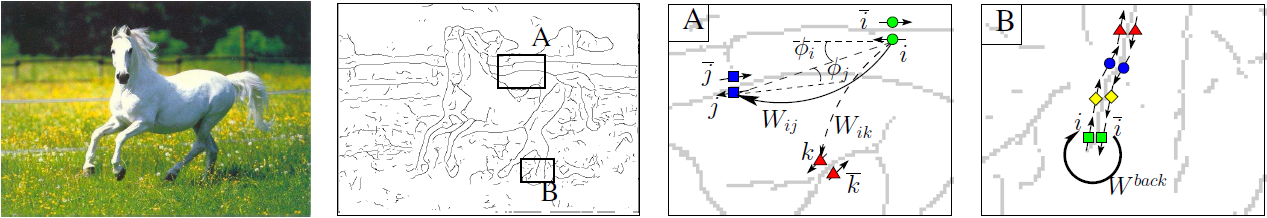
\includegraphics[width=0.95\textwidth]{contour_graph}
\end{figure}
\vfill


%%%%%%%%%%%%%%%%%%%%%%%%%%%%%%%%%%%%%%%%%%%%%%%%%%%%%%%%%%%%%%%%%%%%%%%%%%%%%%%%
\NewPage\headline{Circular Embedding}
\vfill
\begin{itemize}
\item A contour $(C, O)$ consists of a set of vertices $C$ and an ordering function $O: C \rightarrow \left\lbrace 1, ..., \lvert C \rvert \right\rbrace $
\item Each node of the contour is mapped to a point on a complex circle, all other points are mapped to the origin.
\item $x_j = r_je^{i\theta_j}$, $r_j = 1$ if $j \in C$ and 0 otherwise,
\item $\theta_j = O(j)\delta$, where $\delta = \frac{2\pi}{\lvert C \rvert}$ is a phase step.
\end{itemize}
\begin{figure}
	\centering
	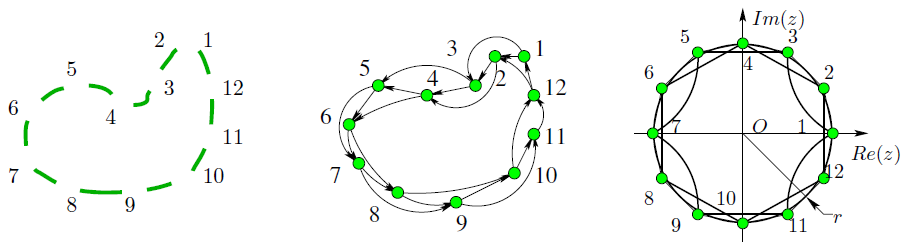
\includegraphics[width=0.8\textwidth]{circular_embedding}
\end{figure}
\vfill


%%%%%%%%%%%%%%%%%%%%%%%%%%%%%%%%%%%%%%%%%%%%%%%%%%%%%%%%%%%%%%%%%%%%%%%%%%%%%%%%
\NewPage\headline{Markov Random Field}
\small
\vfill
\begin{itemize}
\item Nodes are random variables $\left\lbrace x_1, ..., x_n \right\rbrace $ corresponding to pixels.
\item Two types of edges:\\
Correlation between true state and observed data, neighborhood relation
\item A graph represents a joint distribution $p(x)$
\item Can be written as a product of potential functions $\psi_C(x_C)$ over the maximal cliques:
\item[]
	\begin{center}
		$p(x) = \frac{1}{Z} \prod\limits_{C}\psi_C(x_C)$
	\end{center}
\item Conveniently expressed as energy functions: $\psi_C(x_C) = \exp(-E(x_C))$.
\item Can include shape priors into $E$.
\item Maximize $p(x)$ equals to minimize $E$.
\end{itemize}
\begin{table}
  \centering
  \begin{tabular}{@{} M{.5\linewidth} M{.5\linewidth} @{}}
      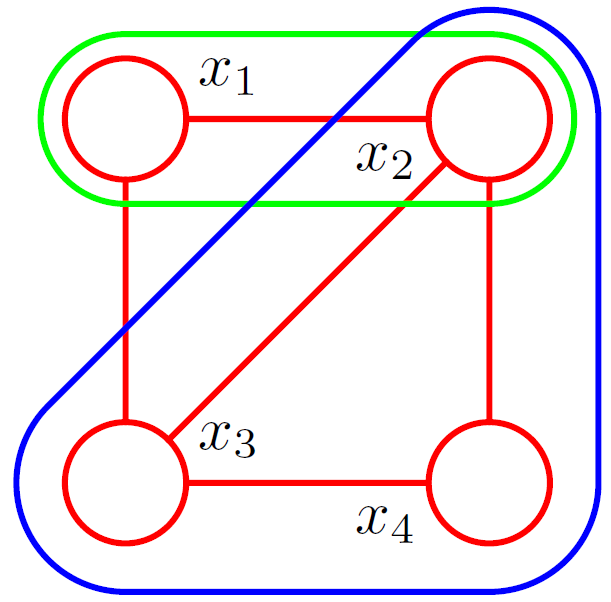
\includegraphics[width=0.15\textwidth]{clique}%
      \caption{Cliques}%
      &
      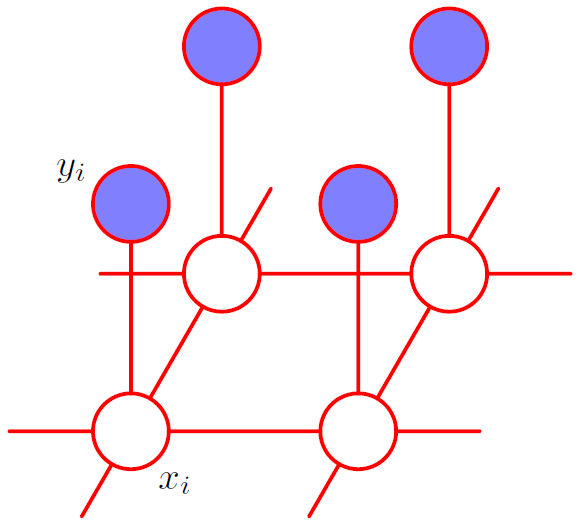
\includegraphics[width=0.15\textwidth]{mrf}%
      \caption{MRF}%
  \end{tabular}
\end{table}
\vfill





%%%%%%%%%%%%%%%%%%%%%%%%%%%%%%%%%%%%%%%%%%%%%%%%%%%%%%%%%%%%%%%%%%%%%%%%%%%%%%%%
\NewPage\headline{Integer Linear Programing formulation of PCST}
\vfill
\begin{itemize}
\item The PCST can be formulated as an ILP problem with $n$ variables and $m$ constraints:
\item[]
\begin{center}
$\max \left\lbrace c^Tx : Ax \geq b, x \in \mathbb{Z}_+^n \right\rbrace $
\end{center}
\item $x \in \mathbb{Z}_+^n$ integer decision variables, $c \in \mathbb{Z}^n$ objective function vector and $A \in \mathbb{Z}^{m \times n}$ the matrix of constraint coefficients.
\item The LP-relaxation (CUT) is obtained by using real-value constraints $x \in \mathbb{R}_+^n$.
\item Its feasible region is the polyhedron:
\item[]
\begin{center}
$P = \left\lbrace x \in \mathbb{R}_+^n : Ax \geq b \right\rbrace $
\end{center}
\item The integral hull of the set of integer solutions, i.e., the polyhedron:
\item[]
\begin{center}
$P_I = \mbox{conv} \left\lbrace x \in \mathbb{Z}_+^n : Ax \geq b \right\rbrace $
\end{center}
%\item A cutting plane as a linear inequality that is valid for $P_I$ but not for $P$.
\item Branch-and-Cut:
\end{itemize}
\begin{table}
  \centering
  \begin{tabular}{@{} M{.5\linewidth} M{.5\linewidth} @{}}
  	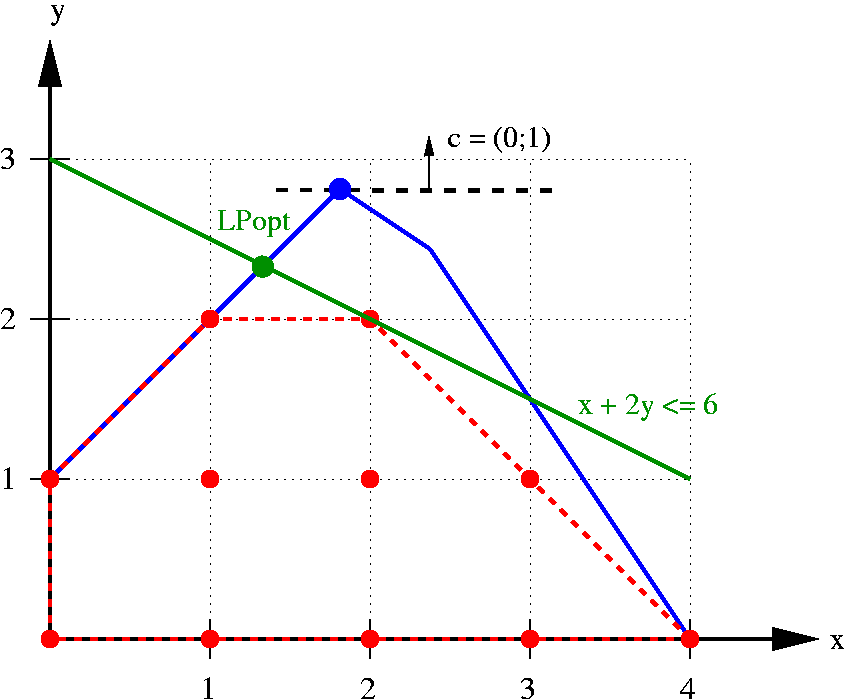
\includegraphics[width=0.2\textwidth]{Cutting_plane_algorithm}
      &
    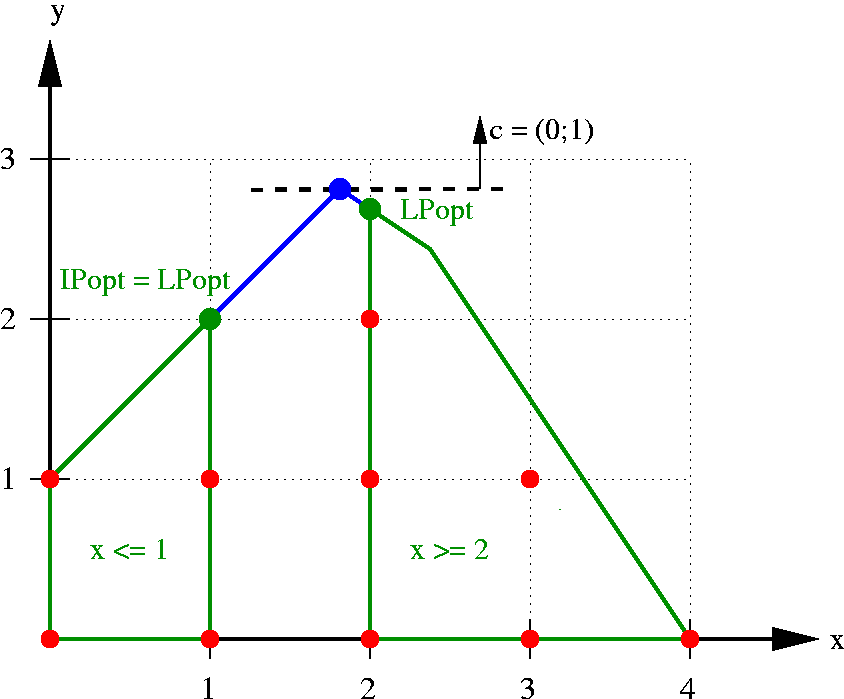
\includegraphics[width=0.2\textwidth]{Branch-and-bound-polytopes}
  \end{tabular}
\end{table}
\vfill









%%%%%%%%%%%%%%%%%%%%%%%%%%%%%%%%%%%%%%%%%%%%%%%%%%%%%%%%%%%%%%%%%%%%%%%%%%%%%%%%
\NewPage\headline{Contour Cut}
\vfill
\begin{itemize}
\item External cut of a contour $(C, O)$ measures its separation from the rest of the graph:
\item[]
\begin{center}
$Ecut(C) = \sum\limits_{i \in C, j \notin C} F_{ij}$
\end{center}
\item Internal cut measures how good it can stay in the form of 1D structure:
\item[]
\begin{center}
$Icut(C, O) = \sum\limits_{(i, j) \in C, \lvert O(i) - O(j) \rvert > k} F_{ij}$
\end{center}
\item The contour cut cost:
\item[]
\begin{center}
$Ccut(C, O) = \dfrac{Icut(C, O) + Ecut(C)}{\mathrm{Vol}(C)}, \qquad \mathrm{Vol}(C) = \sum\limits_{i \in C, (i, j) \in E} F_{ij}$
\end{center}
\item Using circular embedding, $Ccut$ can be transformed into the generalized eigenvalue problem
\end{itemize}
\begin{figure}[htbp]
\centering
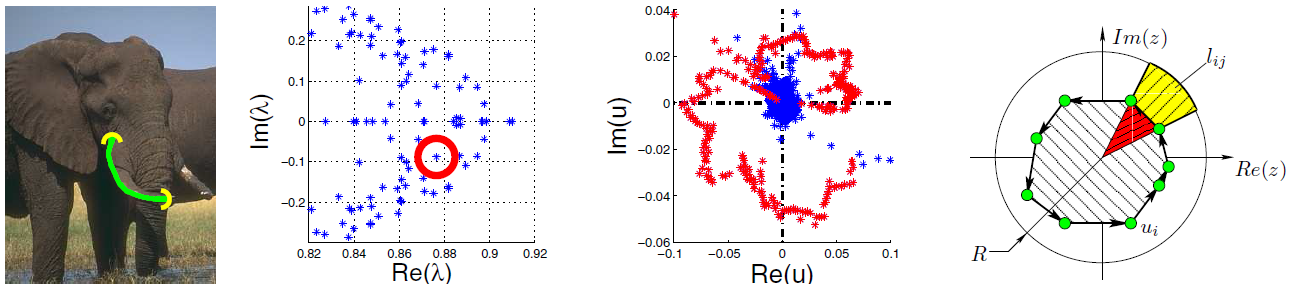
\includegraphics[width=0.9\textwidth]{contour_eigen}
\end{figure}
\vfill





%%%%%%%%%%%%%%%%%%%%%%%%%%%%%%%%%%%%%%%%%%%%%%%%%%%%%%%%%%%%%%%%%%%%%%%%%%%%%%%%
\NewPage\headline{Min-Cut Algorithm}
\vfill
\begin{itemize}
\item MRF $\Rightarrow$ directed weighted graph: terminal nodes $\equiv$ labels, weights $\equiv$ energy.
\item Min-Cut $\equiv$ Max-Flow
\item Augmenting Path Algorithm:
\begin{enumerate}
\item Find path from source to sink with positive capacity
\item Push maximum possible flow through this path
\item Repeat until no path can be found
\end{enumerate}
\end{itemize}
\begin{table}
  \centering
  \begin{tabular}{@{} M{.3\linewidth} M{.3\linewidth} M{.3\linewidth} @{}}
      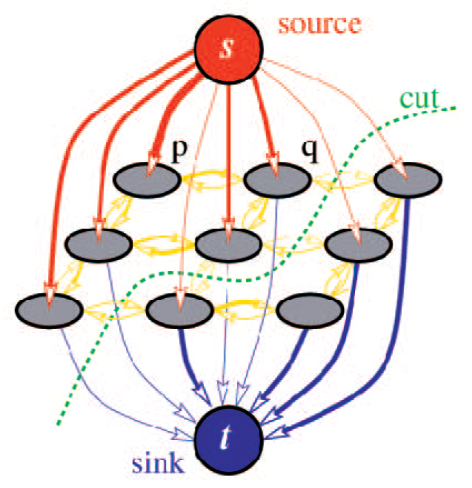
\includegraphics[width=0.3\textwidth]{mincut}%
      &
      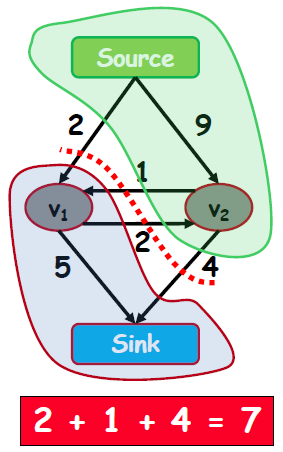
\includegraphics[width=0.2\textwidth]{min_cut}%
      &
      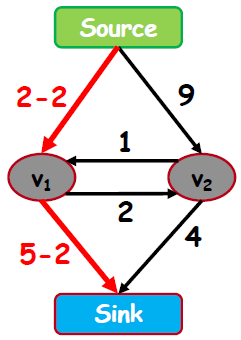
\includegraphics[width=0.2\textwidth]{max_flow}%
  \end{tabular}
\end{table}
\vfill


%%%%%%%%%%%%%%%%%%%%%%%%%%%%%%%%%%%%%%%%%%%%%%%%%%%%%%%%%%%%%%%%%%%%%%%%%%%%%%%%
\NewPage\headline{Multi-Shape Graph-Cut}
\vfill
\begin{itemize}
\item Given 2 labelling configurations $X^0 \in L^{\lvert P \rvert}$ and $X^1 \in L^{\lvert P \rvert}$
\item Fusion move operator of $X^0$ and $X^1$ denoted $X^c = X^0 \odot X^1$:\\
select labels from either $X^0$ or $X^1$ s.t. the energy of $X^c$ is minimized.
\vfill
\item Multi-Shape Graph-Cut Algorithm:
\begin{enumerate}
\item Given current labelling $X^{cur}$, propose label $l$ for background voxels to get $X^{pro}$
\item Fusion two labelling configurations: $X^{cur} \leftarrow X^{cur} \odot X^{pro}$
\item Propose background label for foreground voxels in $X^{cur}$ to get $X^{pro}$
\item $X^{cur} \leftarrow X^{cur} \odot X^{pro}$
\item Until convergence.
\end{enumerate}
\end{itemize}
\vfill


%%%%%%%%%%%%%%%%%%%%%%%%%%%%%%%%%%%%%%%%%%%%%%%%%%%%%%%%%%%%%%%%%%%%%%%%%%%%%%%%
\NewPage\headline{Efficient Region Search (ERS): Datasets}
\vfill
\begin{itemize}
\item PASCAL VOC 2007:
\begin{itemize}
\item Test on two classes: 659 cats and 839 dogs
\item 50\% for training and 50\% for testing
\item Deformable objects with wide pose variation
\item Baseline: Efficient Subwindow Search (ESS)
\end{itemize}
\item ETHZ Shape dataset:
\begin{itemize}
\item 255 images of five shape categories: Applelogos, Bottles, Mugs, Giraffes, Swans
\item Objects are non-boxy
\item 50\% for training and 50\% for testing
\end{itemize}
\item PASCAL VOC 2008 segmentation dataset
\begin{itemize}
\item All 20 categories
\item Baseline: Conditional random field (CRF)
\end{itemize}
\end{itemize}
\begin{table}
  \centering
  \begin{tabular}{@{} M{.25\linewidth} M{.25\linewidth} M{.25\linewidth} M{.25\linewidth} @{}}
      \includegraphics[width=0.15\textwidth]{dog}%
      &
      \includegraphics[width=0.15\textwidth]{cat}%
      &
      \includegraphics[width=0.15\textwidth]{bike}%
      &
      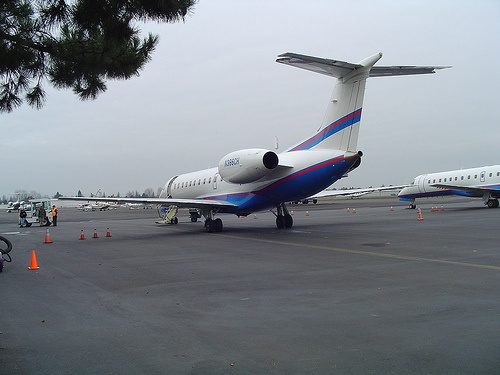
\includegraphics[width=0.15\textwidth]{airplane}%
  \end{tabular}
\end{table}
\vfill


%%%%%%%%%%%%%%%%%%%%%%%%%%%%%%%%%%%%%%%%%%%%%%%%%%%%%%%%%%%%%%%%%%%%%%%%%%%%%%%%
\NewPage\headline{ERS Results}
\vfill
\begin{figure}
	\centering
	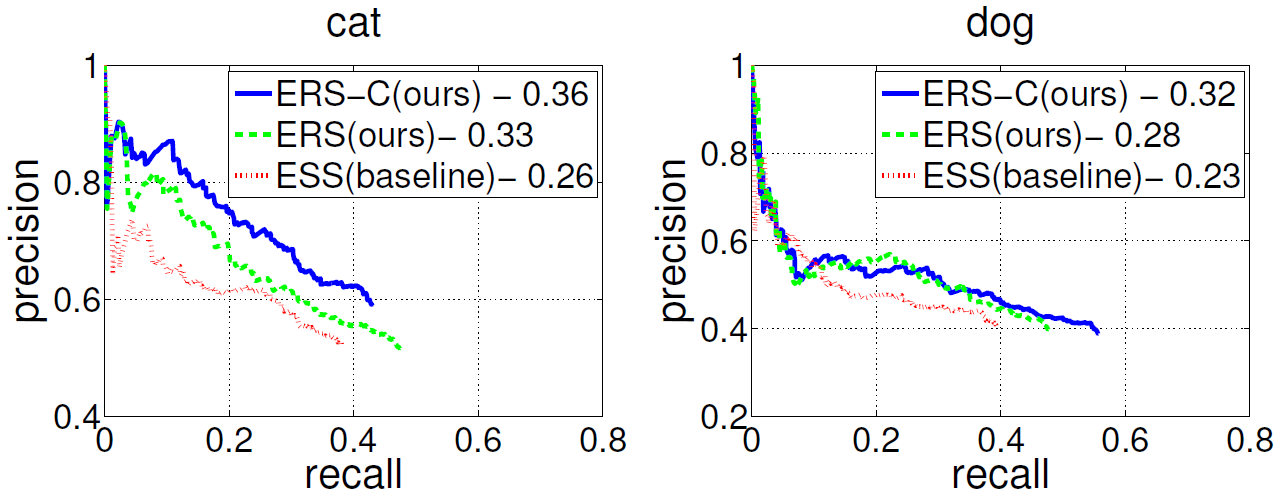
\includegraphics[width=0.45\textwidth]{pascal_voc07}
	\caption{PASCAL VOC 2007}
\end{figure}
\begin{figure}
	\centering
	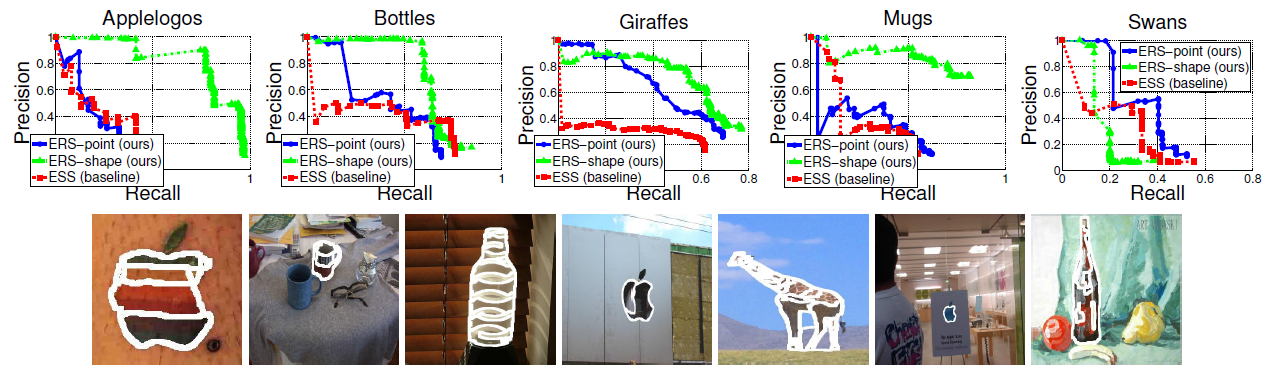
\includegraphics[width=0.75\textwidth]{ERS_result}
	\caption{ETHZ Shape}
\end{figure}
\begin{itemize}
\item PASCAL VOC 2008: mean overlap accuracy 0.274 for ERS vs. 0.228 for CRF
\item Efficiency: 0.29 seconds on average.
\end{itemize}
\vfill


%%%%%%%%%%%%%%%%%%%%%%%%%%%%%%%%%%%%%%%%%%%%%%%%%%%%%%%%%%%%%%%%%%%%%%%%%%%%%%%%
\NewPage\headline{Contour Cut Result}
\vfill
\begin{itemize}
\item Berkeley Segmentation Dataset: 300 images
\item 200 training images, 100 test images
\item Baseline algorithm: probability of boundary (Pb).
\item Contour Cut uses Pb as input.
\end{itemize}
\begin{table}
  \centering
  \begin{tabular}{@{} M{.4\linewidth} M{.3\linewidth} M{.3\linewidth} @{}}
      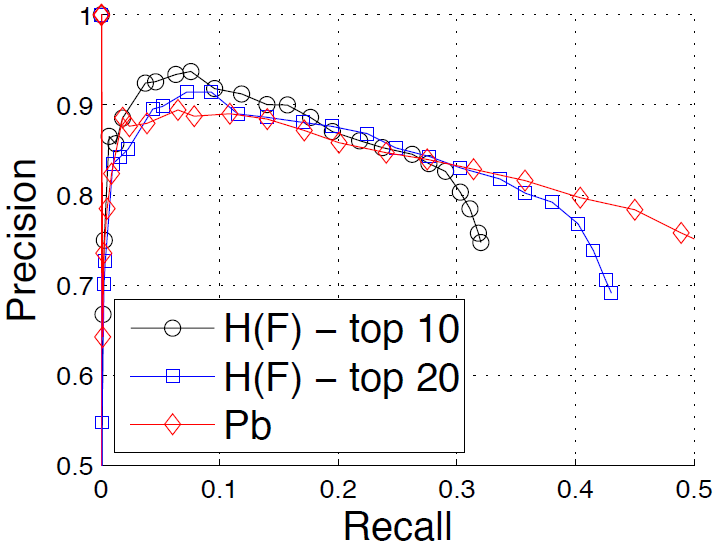
\includegraphics[width=0.4\textwidth]{contour_cut_result}%
      &
      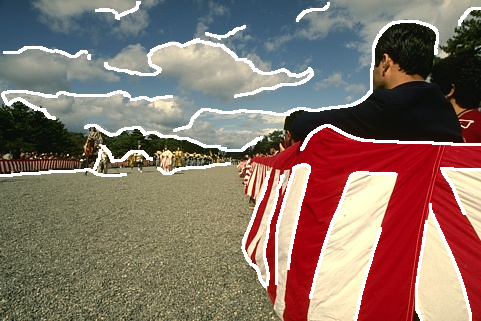
\includegraphics[width=0.3\textwidth]{ccut_result1}%
      &
      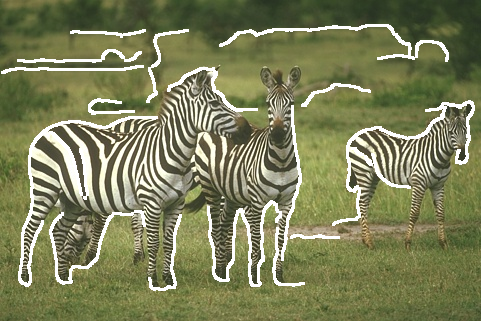
\includegraphics[width=0.3\textwidth]{ccut_result2}%
  \end{tabular}
\end{table}
\vfill


%%%%%%%%%%%%%%%%%%%%%%%%%%%%%%%%%%%%%%%%%%%%%%%%%%%%%%%%%%%%%%%%%%%%%%%%%%%%%%%%
\NewPage\headline{Multi-Shape Graph-Cut Result}
\vfill
\begin{itemize}
\item 97 CT images: 49 for training and 48 for test
\item Baseline algorithm: single-shape graph-cuts
\item Metric: average distance between extracted surface and ground truth.
%\item Average distance of (b) 0.835[mm] vs. (c) 0.523; (e) 0.862 vs. (f) 0.732
\item Efficiency: 30 mins per CT volume (Intel(R) Core(TM) i7 3.07 GHz $\times$ 2)
\item Image sizes: 512 $\times$ 512 $\times$ 204-561[voxel]
\end{itemize}
\begin{figure}
	\centering
	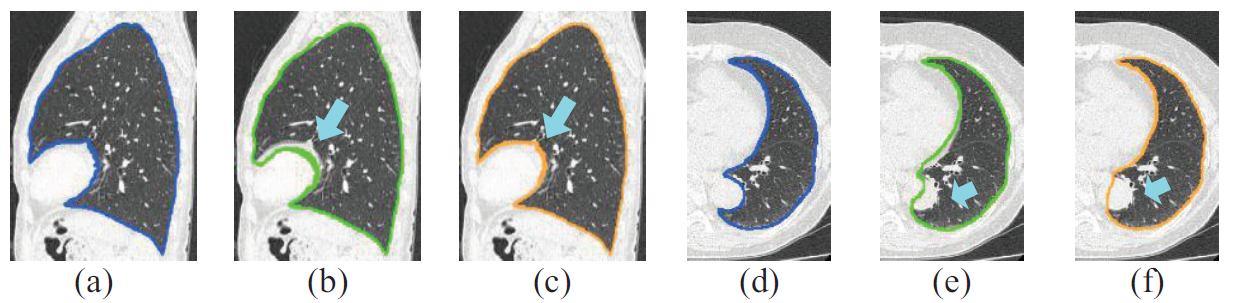
\includegraphics[width=0.9\textwidth]{graphcut_result2}
\end{figure}
\vfill


%%%%%%%%%%%%%%%%%%%%%%%%%%%%%%%%%%%%%%%%%%%%%%%%%%%%%%%%%%%%%%%%%%%%%%%%%%%%%%%%
\NewPage\headline{Multi-Shape Graph-Cut}
\vfill
\begin{figure}
	\centering
	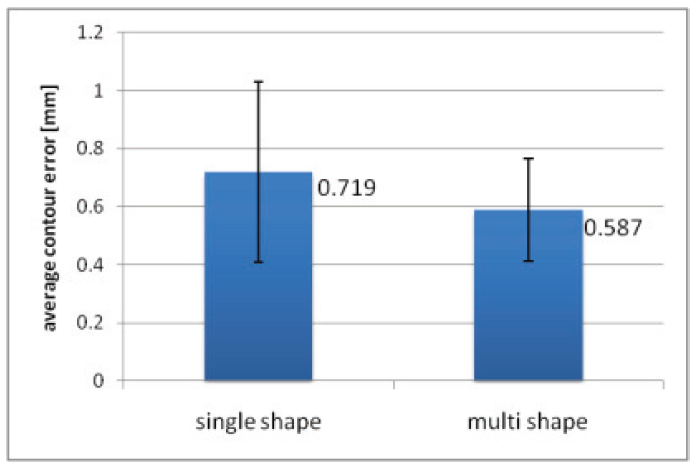
\includegraphics[width=0.35\textwidth]{multi_shape_vs_single}
	\caption{Average distance over all testing data}
\end{figure}
\begin{itemize}
\item Limitation: Results depend on shape priors
\end{itemize}
\begin{figure}
	\centering
	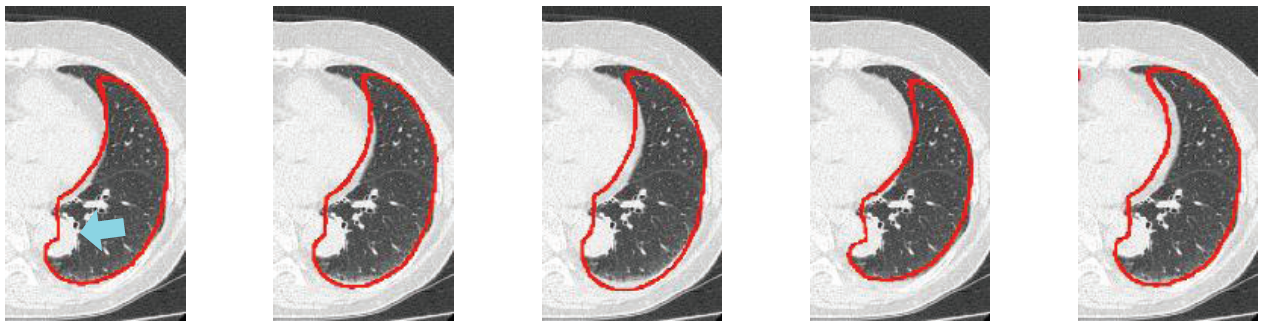
\includegraphics[width=0.85\textwidth]{shape_priors}
\end{figure}
\vfill



%%%%%%%%%%%%%%%%%%%%%%%%%%%%%%%%%%%%%%%%%%%%%%%%%%%%%%%%%%%%%%%%%%%%%%%%%%%%%%%%
\NewPage\headline{Conclusion}
\vfill
\begin{itemize}
	\item Pros:
	\begin{itemize}
		\item Many problems can be transformed into standard graph problems
		\item Can be solved efficiently
		\item Optimal solution possible
	\end{itemize}
	\vfill
	\item Cons:
	\begin{itemize}
		\item ERS only applicable to linear classifiers
		\item Contour Cut is a method to pick up salient contours from Pb edge detector
		\begin{itemize}
			\item If we increase the number of contours, it converges to Pb result
		\end{itemize}
		\item Multi-Shape Graph-Cut depends on shape priors
		\begin{itemize}
			\item Can only extract shapes similar to shape priors
		\end{itemize}
	\end{itemize}
\end{itemize}
\vfill




%%%%%%%%%%%%%%%%%%%%%%%%%%%%%%%%%%%%%%%%%%%%%%%%%%%%%%%%%%%%%%%%%%%%%%%%%%%%%%%%
\FinalPage
%%%



%%%%%%%%%%%%%%%%%%%%%%%%%%%%%%%%%%%%%%%%%%%%%%%%%%%%%%%%%%%%%%%%%%%%%%%%%%%%%%%%
\NewPage
\footnotesize
%\headline{\refname}
%\renewcommand*{\refname}{}
\bibliographystyle{i6bibliostyle}
\bibliography{slides}



%\clearpage
\appendix
%%%%%%%%%%%%%%%%%%%%%%%%%%%%%%%%%%%%%%%%%%%%%%%%%%%%%%%%%%%%%%%%%%%%%%%%%%%%%%%%
\NewPage\headline{\appendixname: Metrics in Information Retrieval}
\vfill
\begin{itemize}
\item $\mathrm{Precision} = \dfrac{\lvert \left\lbrace \mathrm{relevant\ images} \right\rbrace \cap \left\lbrace \mathrm{retrieved\ images} \right\rbrace \rvert}{\lvert \left\lbrace \mathrm{retrieved\ images} \right\rbrace \rvert}$
\item $\mathrm{Recall} = \dfrac{\lvert \left\lbrace \mathrm{relevant\ images} \right\rbrace \cap \left\lbrace \mathrm{retrieved\ images} \right\rbrace \rvert}{\lvert \left\lbrace \mathrm{relevant\ images} \right\rbrace \rvert}$
\item $\mathrm{Average\ Precision} = \dfrac{\sum\limits_{k = 1}^{n} P(k)\cdot rel(k)}{\lvert \left\lbrace \mathrm{relevant\ images} \right\rbrace \rvert}$
\item $P(k): \mathrm{precision\ at\ } k, n: \lvert \left\lbrace \mathrm{retrieved\ images} \right\rbrace \rvert$
\item $rel(k) = \begin{cases} 1, & \mbox{if the image at rank } k\mbox{ is relevant} \\ 0, & \mbox{otherwise} \end{cases}$
\end{itemize}
\vfill



\end{document}
